%##############################################################
\chapter{Grundbegriffe der Regelungstechnik}
%##############################################################
%
Ziel der Regelungstechnik ist eine gegebene Regelgröße $y$ auf einen festgelegten Wert zu bringen. In den meisten Fällen lässt sich diese Regelgröße nicht direkt, sondern nur indirekt durch ein Ventil oder ein anderes technisches Stellglied einstellen. Diese indirekte Beeinflussung erfolgt über die Eingangsgröße $u$ eines Systems und wirkt über die inneren Zustände $x$ auf dessen Ausgang $y$, welcher die Regelgröße darstellt. Die folgende Abbildung \ref{fig:dynamischessystem} stellt ein dynamisches System mit den vorgenannten Größen dar \cite{Foellinger94}.
%
\begin{figure}[h]
	\centering
	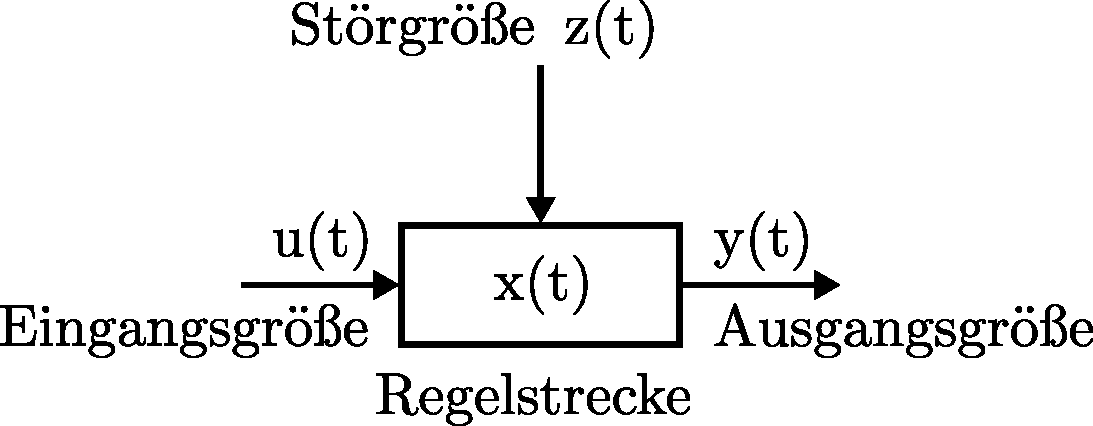
\includegraphics[width=0.5\linewidth]{Abbildungen/Grundbegriffe/PDF/DynamischesSystem.pdf}
	\caption{Dynamisches System als Beschreibung eines physikalischen Prozess}
	\label{fig:dynamischessystem}
\end{figure}
%
In Tabelle \ref{tab:beispieledynsystem} werden einige Beispiele gegeben, welche technische Systeme aus unserem Alltag mit den Kenngrößen aus Abbildung \ref{fig:dynamischessystem} verknüpfen.
%
\begin{table*}[h]\centering
	\ra{1.3}
	\caption{Beispiele für dynamisches Systeme und ihre zugehörigen Systemgrößen}
	\begin{tabular}{@{}llll@{}}\toprule
		Dynamisches System & $u(t)$ & $y(t)$ & $z(t)$ \\ \bottomrule\bottomrule
		Gleichstrommaschine & Ankerspannung & Drehzahl & Lastmoment \\
		Raumheizung & Thermostatstellung & Raumtemperatur & Außentemperatur \\
		Füllstandsregelung & Zugflussventilstellung & Füllhöhe & Abfluss \\
		Noise-Cancelling & Gegenmembran & Signal-Rauschverhältnis & Umgebungsgeräusche\\
		Pupille im Auge & Pupillenweite & Lichteinfall & Krankheiten, Alkohol\\
		Population & Raubtiere & Anzahl der Beutetiere & Jäger (Mensch)\\
		\bottomrule
	\end{tabular}
	\label{tab:beispieledynsystem}
\end{table*}\newpage
%
\textbf{Allgemein gilt:} Die Voraussetzung für den Einsatz einer Regelung ist ein bestenfalls mathematisch beschreibbarer Zusammenhang zwischen $u(t)$ und $y(t)$. Zudem sind weitere Informationen über die Wirkung und den Wert der jeweiligen Größen notwendig.\\\\
%
Schematischer Ablauf einer Regelung \cite{Lunze10}:
\begin{itemize}
	\item[1] Messen der Regelgröße $y(t)$: Dies erfolgt entweder direkt mit einem Sensor, oder wird aus messbaren Größen berechnet.
	\item[2] Vergleich zwischen Führungsgröße $w(t)$ und Regelgröße $y(t)$: Die Differenz dieser beiden Größen wird als Regeldifferenz $e(t)=w(t)-y(t)$ bezeichnet.  
	\item[3] Bestimmung der Stellgröße und Beeinflussung des Eingangs $u(t)$ der Regelstrecke: Dies erfolgt in der Regel unter Berücksichtigung der dynamischen Eigenschaften des Systems. 
\end{itemize}
%
An dieser Stelle sei darauf hingewiesen, dass die Rückführung das zentrale Element der Regelung darstellt \cite{Lunze10}.
%
%###############################################################################
\section{Historische Beispiele der Regelungstechnik}
%###############################################################################
%
\subsection{Antike Wasseruhr}
%
Die ersten praktischen Einsatzgebiete der Regelungstechnik waren mechanische oder fluidmechanische Konstruktionen. 
%
\begin{figure}[h]
	\centering
	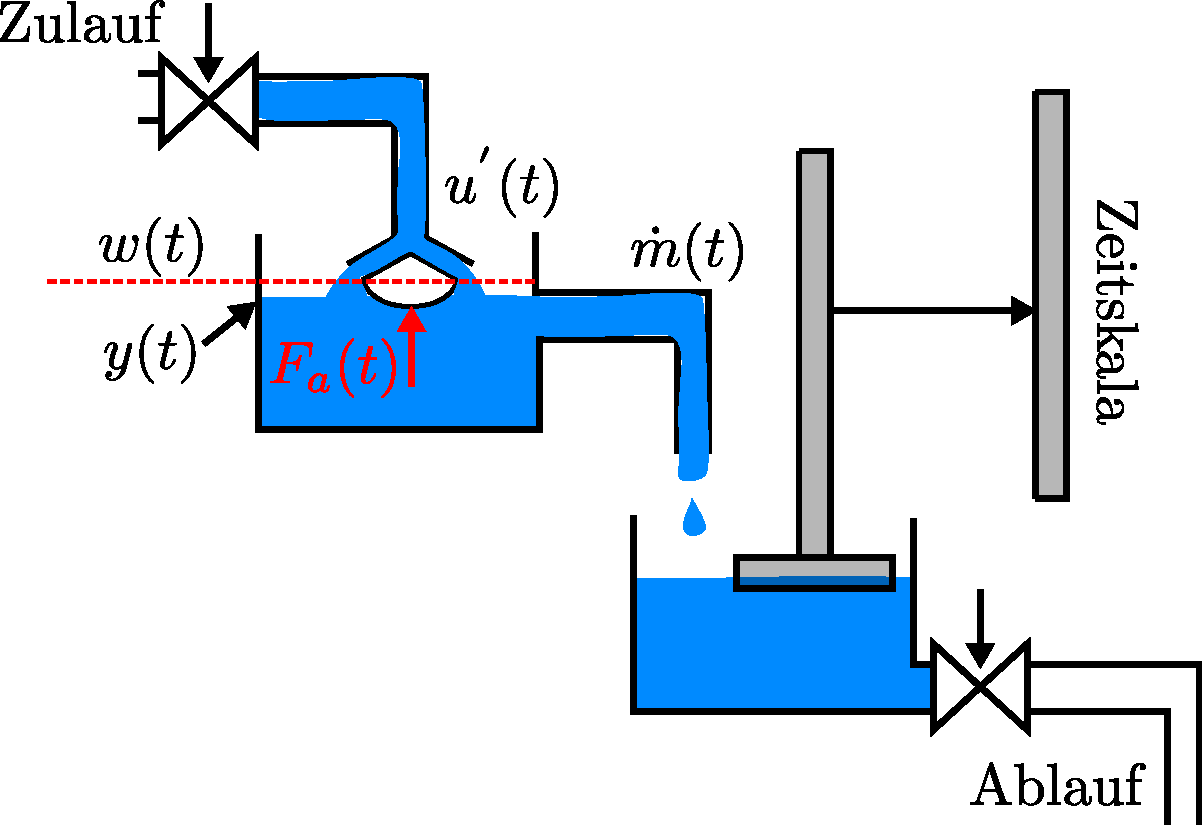
\includegraphics[width=0.6\linewidth]{Abbildungen/Grundbegriffe/PDF/HistorischeSystemeWasseruhr.pdf}
	\caption{Prinzipdarstellung einer antiken Wasseruhr, welche in dieser oder ähnlicher Form zwischen 1500-300 Jahre B.C. zum Einsatz kamen}
	\label{fig:wasseruhr}
\end{figure}
%
Zwar war die Regelungstechnik als solche noch nicht bekannt, ihre Grundprinzipien fanden jedoch schon sehr früh Anwendung, wie z.B. in Wasseruhren \cite{Lewis00,Landes00}. Der prinzipielle Aufbau solch einer Wasseruhr ist in Abbildung \ref{fig:wasseruhr} dargestellt. 
%
Das Regelungsziel war im Falle der Wasseruhr eine gleichmäßige Befüllung des unteren Behälters. Ein Schwimmer mit aufgesetztem Stab bewegt sich durch diese Füllstandsänderung an einer Zeitskala entlang. Je gleichmäßiger sich also der untere Behälter füllt, umso geringer sind die Unterschiede der gezählten Stunden über den Tag. Aus Regelungstechnischer Sicht ist das obere Becken die Regelstrecke:
%
\begin{itemize}
%
	\item Der Wasserzufluss $u^{'}(t)$ wird als konstant angenommen. Der Zufluss $u(t)$ in den oberen Behälter wird durch einen Schwimmer geregelt, welcher durch seine Auftriebskraft relativ zum Pegel als Ventil wirkt.
	%
	\item Somit ist der Sollwert $w(t)$ ein fester Pegel, welcher zu einem vordefiniertem Durchfluss an Wasser $\dot{m}(t)$ führt.
	%
	\item Die Regeldifferenz ergibt sich aus dem Sollwert und dem tatsächlichen Pegel $e(t)=w(t)-y(t)$
	%
	\item Als Eingang auf dass Stellglied (Schwimmer) wirkt die Auftriebskraft $F_{a}(t)$
\end{itemize}
%
\subsection{Fliehkraftregler von James Watt}
%
Ein mechanisches Beispiel wurde von James Watt um 1788 auf der Basis des Prinzips von rotierenden Körpern entwickelt \cite{Unbehauen08}. Der sogenannte Fliehkraftregler war in der Lage, die Drehzahl Watt's Dampfmaschinen zu regeln und so konstant zu halten. Der prinzipielle Aufbau der Regelung ist in Abbildung \ref{fig:fliehkraftregler} dargestellt.
%
\begin{figure}[h]
	\centering
	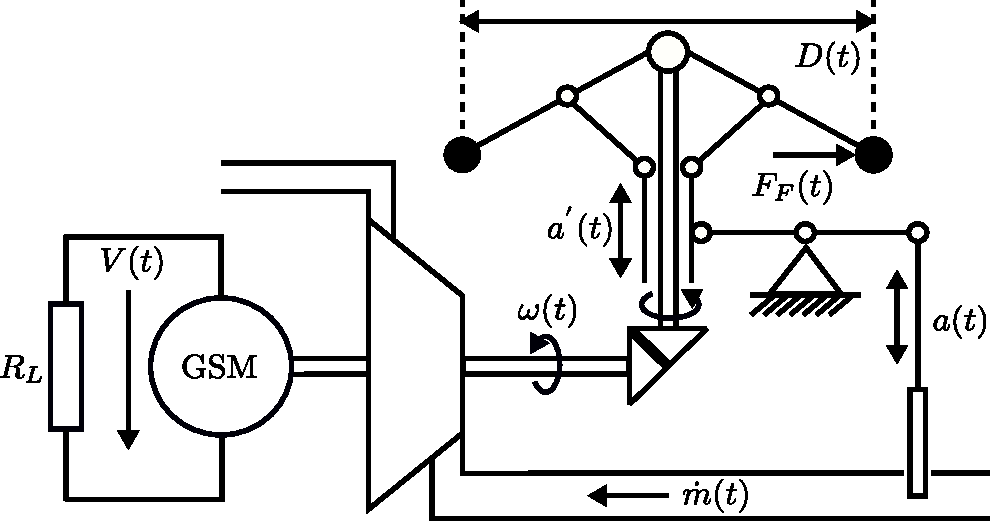
\includegraphics[width=0.83\linewidth]{Abbildungen/Grundbegriffe/PDF/HystorischeSystemeFliehkraft.pdf}
	\caption{Prinzipdarstellung einer Dampfmengenregelung durch einen Fliehkraftregler (Größen der einzelnen Komponenten, nicht maßstabsgetreu)}
	\label{fig:fliehkraftregler}
\end{figure}
%
Auf der linken Seite der Abbildung \ref{fig:fliehkraftregler} ist eine Gleichstrommaschine darstellt, welche im 18 Jahrhundert noch immer für die Generation von Elektrizität genutzt wurde, um Haushalte und die Industrie zu versorgen. Die Ausgangsspannung der Gleichstrommaschine musste für diesen Fall konstant geregelt werden, um eine gleichbleibende Versorgung der angeschlossenen Verbraucher sicherzustellen. Spannungsschwankungen machten sich sofort in der Helligkeit von Glühlampen oder der Drehzahl der angeschlossenen Maschinen in der Industrie bemerkbar. Da die Drehzahl der Gleichstrommaschine (bei Vernachlässigung der Verluste) der Gleichung \ref{eq:gleichstrommaschine}
%
\begin{align}
	V(t) = \phi\,\omega \label{eq:gleichstrommaschine}
\end{align}
%
folgt, kann dies über eine Regelung der Drehzahl erreicht werden. Im rechten Teil der Abbildung \ref{fig:fliehkraftregler} ist der angesprochenen Fliehkraftregler dargestellt. Die Funktion des Reglers kann wie folgt beschrieben werden:
%
\begin{itemize}
%
\item Eine Rotation der Gelenkstangen mit der Kreisfrequenz $\omega(t)$, welche über ein Kegelzahnrad von der Welle der Dampfmaschine angetrieben werden, führt durch die Fliehkraft $F_{F}(t)$ zu einem konstanten Kugelabstand $D(t)$.
%
\item Ändert sich die Kreisfrequenz $\omega(t)$, so ändert sich auch die Fliehkraft $F_{F}(t)$ und somit durch die Gelenkkonstruktion der Abstand $D(t)$ der beiden Gewichte des Reglers.
%
\item Das mechanische Umlenksystem übersetzt den Abstand $D(t)$ über  die Position $a^{'}(t)$ in die Dampfventilstellung $a(t)$.
%
\item Über die Dampfventilstellung $a(t)$ wird die Dampfmenge $\dot{m}(t)$ und somit das Drehmoment bzw. die Drehzahl der Dampfturbine geregelt.  
%
\end{itemize}
%
%
%##############################################################
\subsection{Regelungstechnik in der Neuzeit bis Heute}
%##############################################################
%
Seit den eher intuitiven Ansätzen regelungstechnischer Apparate sind viele mathematische und technische zusammenhänge erforscht worden, die heute einen wesentlich differenzierten und analytischen Blick auf die Regelungstechnik erlauben. Zunächst bedarf es somit einer Einordnung der Analysen und Grundlagenarbeiten, welche im weiteren zur modernen Regelungstechnik geführt haben \cite{Zom13}.
%
\begin{itemize}
	\item 1782 Jozef Maximili\'an Petzval, Pierre-Simon Laplace: \textit{Laplace-Transformation}
	\item 1868 James Clerk Maxwell: \textit{On Governors}, theoretische Betrachtung des Fliehkraftreglers
	\item 1877 Edward J. Routh: \textit{Treatise on the stability of a given state of motion}, Arbeit zum Stabilitätsbegriff linearer Systeme
	\item 1892 Aleksandr M. Lyapunov: \textit{The general problem of the stability of motion}, Verallgemeinerung der Stabilitätsbegriffes für beliebige dynamische Systeme
	\item 1895 Adolf Hurwitz: \textit{Über die Bedingungen unter welchen eine Gleichung nur Wurzeln mit negativen reellen Teilen besitzt.} (Routh-Hurwitz-Kriterium)
	\item 1932 Harry Nyquist: \textit{Regeneration theory}
	\item 1942 J. G. Ziegler, N. B. Nichols: \textit{Optimum settings for automatic controllers}, heuristische Einstellregeln für PID-Regler
	\item 1945 Hendrik W. Bode: \textit{Network analysis and feedback aplifier design}, 
	\item 1961 Rudolf E. K\'alm\'an, Richard S. Bucy: \textit{New results in linear filtering and prediction theory}, der K\'alm\'an Filter begründet den Zeitpunkt der modernen Regelungstechnik
\end{itemize}
%
Besonders durch die theoretischen Arbeiten von Petzval und Laplace in der Laplace-Transformation, aber auch die technischen Untersuchungen zum Fliehkraftregler von Maxwell konnten nun theoretische Konstrukte der Regelungstechnik entwickelt werden. Bis ins Jahr 1940 hatte sich die Regelungstechnik dann zur einer eigenständigen Wissenschaft etabliert. In dieser Vorlesung werden klassische Verfahren der Regelungstechnik eingeführt, welche sich bis 1960 entwickelt hatten.\\\\
%
In der heutigen Zeit ist die Regelungstechnik auch aus unserem Alltag nicht mehr weg zu denken. Unsere batteriebetriebenen Smart-Phones besitzen geregelte Spannungswandler, welche den unterschiedlichen Prozessoren und Komponenten bedarfsgerecht ihre Versorgung bereitstellen. Moderne Personen-Kraft-Wagen (PKW) besitzen Geschwindigkeitsregeleinrichtungen, um per Knopfdruck eine gewisse Fahrgeschwindigkeit einzustellen. 
%
%\footnote{Schottischer Mathematiker/Physiker. Hat die Theorie der Elektrodynamik entwickelt, und somit als erster Mensch den Zusammenhang %zwischen Elektriziät und Magnetismus mathematisch beschrieben. Die Hauptergebnisse seiner Arbeit sind als Maxwellsche Gleichungen bekannt %\cite{Maxwell54}.} 
%
\newpage
%
%##############################################################
\section{Struktur einer Regelung}
%##############################################################
%
%##############################################################
\subsection{Vollständiger Wirkungsplan einer Regelung}
%##############################################################
%
Grundsätzlich gibt es mehrere Möglichkeiten, um eine Regelung zu beschreiben. Zum einen kann sie durch das Aufstellen von mathematischen Gleichungssystemen erfolgen. Dies ist in den meisten Fällen zwar notwendig, jedoch für die strukturelle Aufbereitung zunächst nicht Zielführend. Deshalb wird an dieser Stelle der Wirkungsplan einer Regelung nach DIN IEC 60050-351 (ehemals DIN 19226-4) \cite{DKE14} eingeführt (vlg. Abbildung~\ref{fig:regelkreisdin}).
%
\begin{figure}[h]
	\centering
	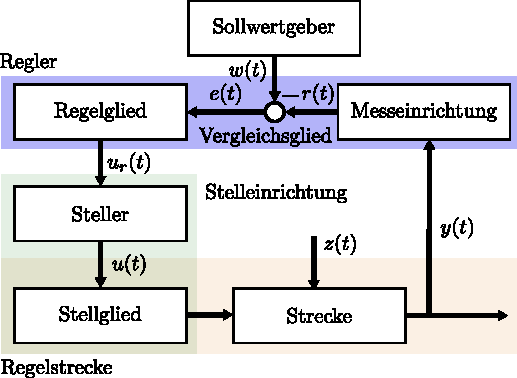
\includegraphics[width=0.70\linewidth]{Abbildungen/Grundbegriffe/PDF/VollstWirkungsplan.pdf}
	\caption{Wirkungsplandarstellung einer Regelung nach DIN}
	\label{fig:regelkreisdin}
\end{figure}\\
%
Folgende Begrifflichkeiten sollen hier näher erläutert werden (siehe auch\cite{Foellinger94}\cite{MSF05}):
\begin{itemize}
\item Systemblock Regeleinrichtung
\begin{description}
\item \underline{Messeinrichtung:} Hat die Aufgabe, die allgemeine Messgröße (Weg, Strom, Drehzahl, Druck) in eine für das Regelungssystem verarbeitbare Form umzuwandeln. Hierbei muss beachtet werden, dass Messglieder auch ein Übertragungsverhalten besitzen.
%
\item \underline{Sollwertgeber:} Erzeugt die Führungsgröße des Regelkreises und gibt sie an die Vergleichsstelle zwischen Messeinrichtung und Regelglied weiter
\item \underline{Vergleichsglied:} Bildet die Regeldifferenz $e(t)$ aus Ausgangsgröße $y(t)$ und Sollwert $w(t)$.
\item \underline{Regelglied:} Dieser Teil der Regeleinrichtung berechnet aus der Regeldifferenz $e(t)$ eine Referenzgröße für den Steller. Dieser Berechnung liegt das Regelgesetz zugrunde.
\end{description}
%
\item Systemblock Stelleinrichtung
\begin{description}
	\item \underline{Steller:} Ist die ausführende Funktionseinheit und wandelt das Ausgangssignal des Regelglieds in ein für das Stellglied verständliches Signal um.
	%
	\item \underline{Stellglied:} Ist meist Teil der Regelstrecke und setzt das Stellsignal um, indem es in die zu regelnden Größen $\boldsymbol{x}(t)$ eingreift. 
\end{description}
%
\item Systemblock Regelstrecke
\begin{description}
	\item \underline{Strecke:} Ist der Teil des Regelkreises, in welchem sowohl die Regelgrößen beeinflusst, als auch die Messgrößen abgegriffen werden. Oft wird die Regelstrecke auch als der zu regelnde Prozess bezeichnet.
\end{description}
\end{itemize}
%
%##############################################################
\subsection{Vereinfachter Wirkungsplan einer Regelung}
%##############################################################
%
Wird die Messeinrichtung und das Stellglied als Teil der Regelstrecke angesehen und der Steller in die Regeleinrichtung integriert, ergibt sich das folgende vereinfachte Blockschaltbild (vgl. Abbildung~\ref{fig:regelkreiseinfach}), welches den Wirkungsplan auf seine wesentlichen Komponenten vereinfacht \cite{MSF05}. 
%
\begin{figure}[h]
	\centering
	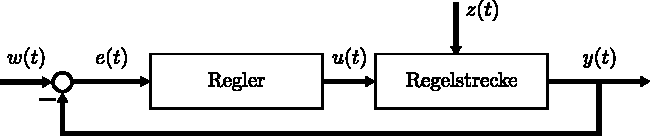
\includegraphics[width=0.9\linewidth]{Abbildungen/Grundbegriffe/PDF/VereinfWirkungsplan.pdf}
	\caption{Vereinfachte Wirkungsplandarstellung}
	\label{fig:regelkreiseinfach}
\end{figure}\\ 
%
Das Regelglied wird nun vereinfacht als 'Regler' bezeichnet und die Regelstrecke enthält nun die Messeinrichtung so wie das Stellglied.
%
%##############################################################
\subsection{Wirkungsplan am Beispiel einer Fahrstuhlregelung}
%##############################################################
%
Die Vorgehensweise zur Aufstellung des vollständigen und vereinfachten Wirkschaltplanes, soll nun Anhand einer Drehzahlregelung einer Gleichstrommaschine dargestellt werden (aus \cite{MSF05}, Beispiel 1.9). In Abbidung~\ref{fig:aufzug} ist zunächst der technische Prozess mit den jeweiligen Komponenten dargestellt.
%
\begin{figure}[ht!]
	\centering
	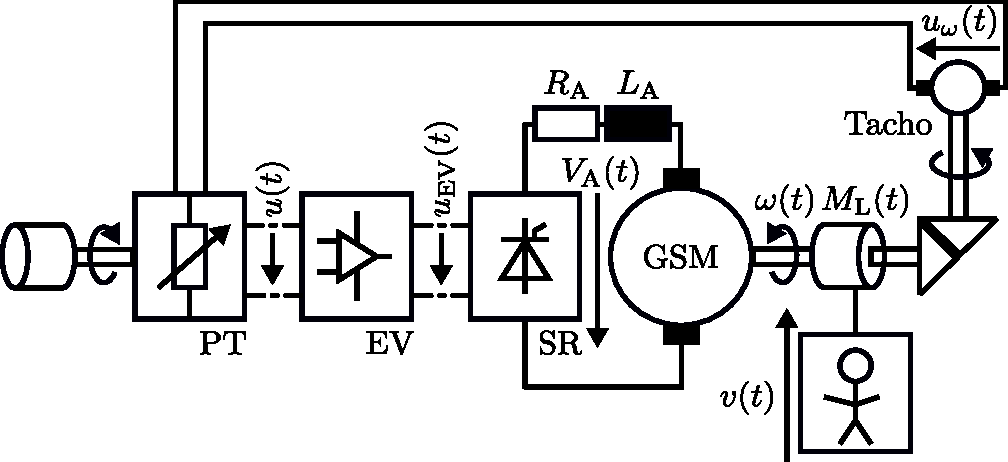
\includegraphics[width=0.83\linewidth]{Abbildungen/Grundbegriffe/PDF/Fahrstuhlregelung.pdf}
	\caption{Regelung der Fahrgeschwindigkeit eines Aufzuges (nach \cite{MSF05} Bild 1.14 a) )}
	\label{fig:aufzug}
\end{figure}
%
\begin{Aufgaben}{}{}
	\begin{itemize}
		\item \textit{Blockschaltbild der Fahrstuhlregelung}
	\end{itemize}
\end{Aufgaben}
%
Wird nun der technische Prozess durch seine Wirkungsblöcke dargestellt, ergibt sich folgender vollständiger Wirkungsplan (Abbildung~\ref{fig:aufzugwirkvoll}).  
%
\begin{figure}[ht!]
	\centering
	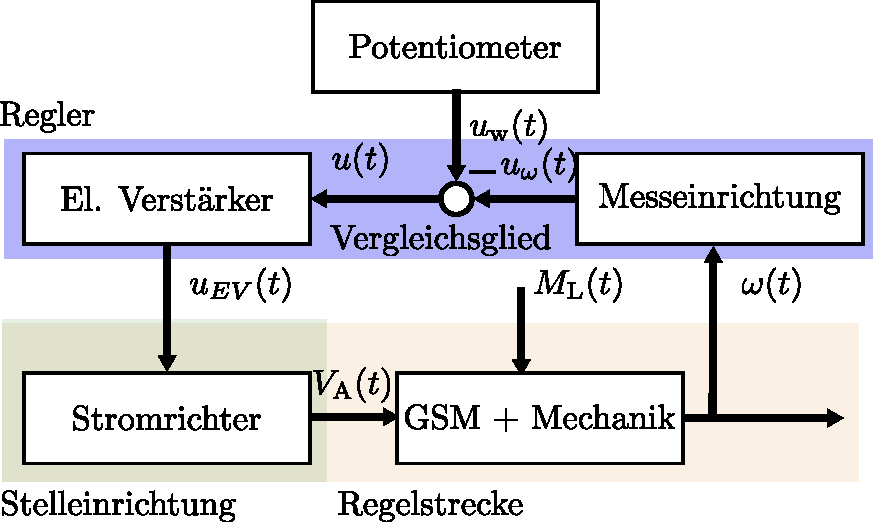
\includegraphics[width=0.7\linewidth]{Abbildungen/Grundbegriffe/PDF/FahrstuhlregelungWirkungsplan.pdf}
	\caption{Vollständige Wirkungsplandarstellung der Fahrstuhlregelung (nach \cite{MSF05} Bild 1.14 b)}
	\label{fig:aufzugwirkvoll}
\end{figure}
%
Durch die Kombination von Stromrichter, Gleichstrommotor, Aufzug und Tachogenerator ergibt sich der vereinfachte Wirkungsplan der Fahrstuhlregelung. Der Vorgang wird an dieser Stelle nicht weiter ausgeführt, da er dem allgemeinen Prinzip folgt.
%
%#########################################################################################################
\section{Prinzip der Steuerung in der offenen Wirkungskette}
%#########################################################################################################
%
Eine Steuerung wird meist als offene Wirkungskette bezeichnet und besitzt keine Rückführung der Regelgröße, wie in Abbildung~\ref{fig:steuerung} dargestellt.
%
\begin{figure}[h]
	\centering
	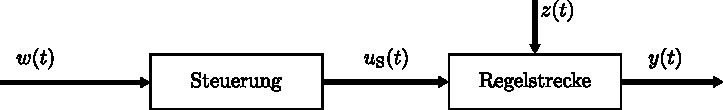
\includegraphics[width=0.95\linewidth]{Abbildungen/Grundbegriffe/PDF/Steuerung.pdf}
	\caption{Prinzip der Steuerung in der offenen Wirkungskette ohne Rückführung}
	\label{fig:steuerung}
\end{figure}
%
Grundsätzlich kann die Zielvorgabe, nämlich eine Regelgröße auf einen bestimmten Wert einzustellen, auch ohne Rückführung erreicht werden. Sind sämtliche Störungen abgeklungen oder vernachlässigbar $z(t)=0,\forall t \in\{0+,\cdots,\infty\}$, so kann über die Beziehung \eqref{eq:steuerung}
%
\begin{align}
y(t) = f(u(t))\label{eq:steuerung}
\end{align}
%
Berechnet werden, welche Führungsgröße $w(t)$ die Stellgröße $u(t)$ so beeinflusst, dass \eqref{eq:führung} gilt
%
\begin{align}
w(t) = y(t)\label{eq:führung}
\end{align}
%
Dies ist in vielen Fällen nur schwer möglich, da $f(\cdot)$ meist durch eine Differentialgleichung beschrieben werden muss. Das inverse Modell kann nur erstellt werden, wenn die dynamischen Eigenschaften der Regelstrecke ausreichend bekannt sind. Eine Steuerung kann in diesem Fall erstellt werden durch die Vorschrift \eqref{eq:inversion}. 
%
\begin{equation}
\begin{aligned}
u(t) &= f^{-1}(w(t))\\
y(t) &= f(u(t))=f\left(f^{-1}(w(t))\right)=w(t)\label{eq:inversion}
\end{aligned}
\end{equation}
%
Jedoch ist es möglich, dass die Funktion $f^{-1}(\cdot)$ nicht existiert, da $f(\cdot)$ nicht invertierbar ist. Ist dies der Fall, kann nur eine Annäherung $\tilde{f}^{-1}(\cdot)$ berechnet werden. Diese Näherung bewirkt, dass nur die Forderung $y(t)\approx w(t)$ erreicht werden kann.\\
%
Es wir somit recht schnell klar, dass die Regelung wesentliche Vorteile gegenüber einer Steuerung in der offenen Wirkungskette besitzt. Vor allem ist hier jedoch die Sollwertfolge zu nennen, deren Funktion in der geschlossen Wirkungskette trotz unterschiedlicher Eigenschaften der Regelstrecke erhalten bleibt \cite{Lunze10}. Eine Regelung hat grundsätzlich Vorteile:
%
\begin{itemize}
	\item im Falle einer instabilen Regelstrecke.
	\item bei nicht messbaren Störungen. 
	\item falls die statischen und dynamischen Parameter der Strecke nicht genau bekannt sind.
	\item falls diese Parameter sich zeitlich ändern.
\end{itemize} 
%
%#########################################################
\subsection{Anwendung im Regelkreis als Vorsteuerung}
%#########################################################
%
Nichts desto trotz findet das Prinzip der Steuerung in der offenen Wirkungskette in moderne Regelkreise Einzug. Ein Beispiel hierfür ist die Vorsteuerung, welche als weiterer Freiheitsgrad der Regelung genutzt werden kann, um Sollwerte schneller zu erreichen \cite{Lunze10}. Sowohl der Regler als auch die Vorsteuerung erhalten den gleichen Sollwert $w(t)$ und schalten diesen unterschiedlich auf die Strecke auf, wie in Abbildung~\ref{fig:vorsteuerung} dargestellt.
%
\begin{figure}[h]
	\centering
	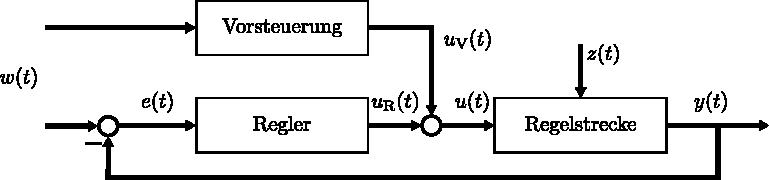
\includegraphics[width=0.95\linewidth]{Abbildungen/Grundbegriffe/PDF/Vorsteuerung.pdf}
	\caption{Nutzung einer Steuerung, um die Sollwertfolge im geschlossenen Regelkreis zu verbessern}
	\label{fig:vorsteuerung}
\end{figure}
%
Die Eingangsgröße $u(t)$ auf die Regelstrecke teilt sich nun in einen Anteil des Reglers $u_{\text{R}}(t)$ und in einen Anteil der Vorsteuerung $u_{\text{V}}(t)$ auf.
%
Beide Kreise können separat entworfen werden, wobei beim Regelkreis nun das Augenmerk auf die Stabilisierung und Störkompensation und bei der Vorsteuerung auf eine möglichst gute Sollwertfolge gelegt wird.\\

\textbf{Eigenschaften:}
\begin{itemize}
	\item Verbessert die Umschaltung zwischen zwei Arbeitspunkten.
	\item Erhöht die Freiheitsgrade in der Regelung.
	\item Sollwert kann meist schneller erreicht werden, als im Falle der 'einfachen' Regelung. 
\end{itemize}
%
%#########################################################
\subsection{Anwendung im Regelkreis als Störgrößenaufschaltung} 
%#########################################################
%
Ein weiteres Anwendungsfeld einer Steuerung ist die Störgrößenaufschaltung oder auch Störgrößenkompensation genannt \cite{Foellinger94,Lunze10}. Zu beachten ist, dass diese nur entworfen werden kann, wenn die zu kompensierenden Störungen $\tilde{z}(t)$ messbar sind \underline{bevor} sie auf die Regelstrecke wirken. Die Störgrößenkompensation im Regelkreis ist in Abbildung~\ref{fig:stoergroesse} dargestellt.
%
\begin{figure}[h]
	\centering
	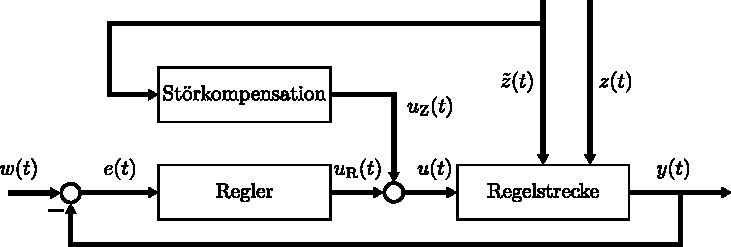
\includegraphics[width=0.95\linewidth]{Abbildungen/Grundbegriffe/PDF/StoerGroessen.pdf}
	\caption{Nutzung einer Störgrößenaufschaltung, um messbare Störung zu kompensieren.}
	\label{fig:stoergroesse}
\end{figure}
%
Ziel der Kompensation ist eine möglichst gute Unterdrückung der Störungswirkung $\tilde{z}(t)$ ohne das Führungsverhalten des Regelkreises wesentlich zu beeinflussen. Grundsätzlich kann jeder Regler auf Führungs- und Störverhalten optimiert werden, aber die Störunterdrückung ist in vielen Fällen effektiver.\\

\textbf{Eigenschaften:}
\begin{itemize}
	\item Realisierbar für Störungen die sich einfach messen lassen.
	\item Wirkung der Störung auf den Regelkreis kann unterdrückt werden.
	\item Eine 100\% Unterdrückung ist praktisch nicht möglich, da dynamische Systeme nicht invertierbar sind.
\end{itemize}
%
\begin{simulation}{}{}
	\begin{itemize}
		\item \textit{Kurze Einführung in Octave}
	\end{itemize}
\end{simulation}
%
%#########################################################
\section{Klassifikation von Regelungsaufgaben}
%#########################################################
%
%#########################################################
\subsection{Festwert- oder Störgrößenregelung}
%#########################################################
\label{sec:Klassifikation}
%
Eine Regelung kann zunächst durch ihre vorrangige Aufgabe klassifiziert werden. Diese Aufgabe kann z.B. die Störgrößenregelung bzw. Festwertregelung sein \cite{MSF05,Zacher17}. Dies bedeutet, dass der Sollwert der zu regelnden Strecke sich nicht wesentlich ändert. Jedoch sind immer wieder Störungen $z(t)$, welche auf die Strecke wirken, zu erwarten. Der Regelkreis sollte in diesem Fall ein gutes Störverhalten aufweisen. Die Systemantwort $h_{\text{z}}(t)$ auf eine Störgröße ist in Abbildung~\ref{fig:festwert} dargestellt.
%
\begin{figure}[h]
	\centering
	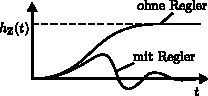
\includegraphics[width=0.4\linewidth]{Abbildungen/Grundbegriffe/PDF/FestwertRegelung.pdf}
	\caption{Typisches zeitliches Verhalten der Störsprungantwort $h_{\text{z}}(t)$, für den Fall ohne und mit Regelung}
	\label{fig:festwert}
\end{figure}
%
Es ist deutlich zu erkennen, dass ohne Regler eine bleibende Abweichung entstehen würde. Diese Abweichung ist im Regelkreis nicht erwünscht und sollte durch die geeignete Wahl des Reglers unterdrückt werden.
%
%#########################################################
\subsection{Folgereglung}
%#########################################################
%
Ändert der Sollwert sich zeitlich, so kann der Regelkreis als Folgeregelung entworfen werden. Die Regelungsaufgabe ist nun, die Regelgröße $y(t)$ dem Sollwert $w(t)$ nachzuführen. Die qualitative Beurteilung der Funktion erfolgt anhand des Führungsverhaltens des Regelkreises \cite{Lunze10}. 
%
\subsubsection{Führungssprungantworten und unterschiedliche Führungsgrößen}
%
Eine klassische Führungsgrößenänderungen ist die Sprungfunktion. Eine CNC-Fräse soll eine neue Position anfahren. Hierfür müssen die Servomotoren ohne Überschwingen und ohne bleibende Regelabweichung auf die neue Zielposition verfahren werden. Andernfalls würde zu viel oder zu wenig Material aus dem Werkstück gefräst werden. In Abbildung~\ref{fig:sprungantwort} ist dieser Sachverhalt exemplarisch dargestellt.
%
\begin{figure}[h]
	\centering
	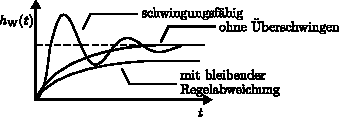
\includegraphics[width=0.65\linewidth]{Abbildungen/Grundbegriffe/PDF/Fuehrungssprung.pdf}
	\caption{Typisches zeitliches Verhalten der Führungssprungantwort $h_{\text{w}}(t)$, für unterschiedliche Reglerparameter}
	\label{fig:sprungantwort}
\end{figure}\\
%
Jedoch ist es gerade bei Servomotoren üblich, die Position mittels einer festgelegten Bahn zu erreichen. In diesem Fall kann eine lineare Änderung der Führungsgröße erfolgen, um den neuen Arbeitspunkt anzufahren. Das Verhalten des Regelkreises mit und ohne bleibende Regelabweichung ist in Abbildung~\ref{fig:anstiegsfunktion} dargestellt.
%
\begin{figure}[h]
	\centering
	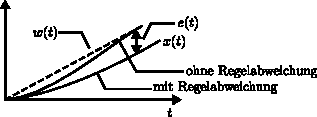
\includegraphics[width=0.65\linewidth]{Abbildungen/Grundbegriffe/PDF/Anstiegsfunktion.pdf}
	\caption{Lineare Führungsgrößenänderung $w(t)$}
	\label{fig:anstiegsfunktion}
\end{figure}
%
Eine weitere in der Praxis genutzte Führungsgröße ist die Parabelform. Diese Parabelform ist beispielsweise bei Industrierobotern zu finden \cite{Lunze10}. Die Position wird dort in Form eines Polynoms vorgegeben und muss durch den Regler eingehalten werden. In vielen Fällen wird diese Aufgabe durch die Kombination mit einer Vorsteuerung gelöst. Das prinzipielle Verhalten ist in Abbildung~\ref{fig:parabelfunktion} dargestellt.
%
\begin{figure}[h]
	\centering
	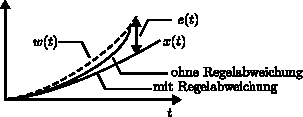
\includegraphics[width=0.65\linewidth]{Abbildungen/Grundbegriffe/PDF/Parabelfunktion.pdf}
	\caption{Parabelförmige Führungsgrößenänderung $w(t)$}
	\label{fig:parabelfunktion}
\end{figure}
%
\underline{Anmerkung:} Es gibt Anwendungen, bei denen trotz der Nutzung einer linearen oder polynomförmigen Führungsgröße keine bleibende Regelabweichung zulässig ist.  
\begin{itemize}
	\item Fliegende Schere: Durchschneiden einer sich bewegenden Papierbahn.
	\item Wiederholgenauigkeit von Trajektorien bei Industrierobotern in der Automobilfertigung.
\end{itemize}
%
\begin{Summary}{}{}
	\begin{itemize}
	\item \textit{Welche Komponenten sind im Regelkreis nach DIN enthalten?}
	\begin{itemize}
		\item \textit{Zeichnen und benennen Sie sämtliche Komponenten}
		\item \textit{Kreisen Sie die jeweiligen Gruppen ein}
	\end{itemize}
	\item \textit{Was ist der Unterschied zwischen offener Wirkungskette und geschlossenem Regelkreis?}
	\item \textit{Für welche Anwendungszwecke kann eine Steuerung eingesetzt werden?}
	\begin{itemize}
		\item \textit{Suchen sie zwei technische Beispiele für Vorsteuerungen aus gängiger Literatur}
	\end{itemize}
	\item \textit{Wie können Regelungsaufgaben grundsätzlich klassifiziert werden?}
	\item \textit{Welche Auswirkungen haben bleibende Regelabweichungen?}
	\end{itemize}
\end{Summary}
%
%%#######################################################################
%\section{Qualitative and Quantitative Anforderungen and den Regelkreis}
%%#######################################################################
%%
%Bisher wurden die notwendigen Begriffe und die Wirkungsweise der Regelung eingeführt. Nun stellt sich die Frage wie eine Regelung zu entwerfen ist. Hierfür müssen zunächst die Anforderungen definiert und spezifiziert werden.
%%
%\subsection{Der Regelkreis als Entwurfsaufgabe}
%%
%Grundsätzlich können die Anforderungen an einen Regelkreis in vier Hauptgruppen unterteilt werden \cite{Lunze10}
%%
%\begin{itemize}
%	\item Stabilität
%	\item Störkompensation und Sollwertfolge
%	\item Dynamisches Verhalten
%	\item Robustheit 
%\end{itemize}